%************************************************
\chapter{Patterns of sitewise selection in mammalian protein-coding genes}\label{ch:mammals1}
%************************************************

\section{Introduction}

\subsection{The Mammalian Genome Project}

A major goal of mammalian comparative genomics has been to quantify,
identify and understand the fraction of the human genome that is under
evolutionary constraint. The first non-human mammalian genomes showed
at least 5\% of the human genome to be under purifying selection
\citep{Mouse2002Initial,Rat2004Genome,LindbladToh2005Genome}, but the
small number of genomes available limited the extent to which regions
of evolutionary constraint could be identified. The \mgp, a
coordinated set of genome sequencing projects initiated in 2005 and
organised by the Broad Institute of MIT and Harvard, was designed with
the primary purpose of increasing the accuracy and confidence with
which regions of the human genome that have evolved under evolutionary
constraint in mammals could be identified \citep{TODO}. In line with
this goal, 20 mammalian species were chosen for sequencing in order to
maximise the amount of evolutionary divergence available for
comparative analysis when combined with the 9 already available
sequenced genomes \citep{Margulies2005Initial}. To save on sequencing
costs most of the 20 additional species were only sequenced to a
target twofold coverage, meaning each genomic base pair would be
covered on average by two sequence reads and roughly 85\% of genomic
sequence would be covered by at least one read.

As the \mgp proceeded from its sequencing to analysis phase in late
2008, it became clear that the additional branch length afforded by
the 29-species phylogeny would enable a number of improved
evolutionary analyses beyond the identification of constrained
noncoding regions. Among others, these included the evolutionary
characterisation of gene promoters, identification of exapted
noncoding elements, detection of evolutionary acceleration and
deceleration in noncoding regions, and detection of purifying and
positive selection in protein-coding genes. Given its prior
involvement in analysing the ENCODE comparative sequencing data
\citep{TODO} and Massingham's work on a method and software program
for sitewise evolutionary analysis \citep{TODO}, the Goldman group
became involved in the protein-coding evolutionary analysis for the
\mgp. This chapter describes my work on the project, which began in
late 2008; the major results from the analysis are to be published in
\citep{TODO}, and all of the work described below was performed by me
in consultation with members of the Goldman group (Nick Goldman and
Tim Massingham), EnsEMBL team (Albert Vilella, Javier Herrero, Ewan
Birney) and organisers and members of the \mgp (Manolis Kellis,
Kerstin Lindblad-Toh, Mike Lin, Katie Pollard).

\subsection{The Sitewise Likelihood Ratio test}

As described in Chapter \ref{ch_bg}, differential survival of \nsyn
and \syn mutations based on the degeneracy of the genetic code can be
used as a source of information on the continued importance of
mutations at a given protein-coding site over evolutionary time: a
lower rate of \nsyn substitution compared to \syn substitution is
indicative of purifying selection, or natural selection in favor of
maintaining protein structure and function; equal rates of \nsyn and
\syn substitutions is indicative of neutral selection, or no
differential survival of protein-altering mutations; a greater rate of
\nsyn than \syn substitution is indicative of positive selection, or
natural selection in favor of protein-altering mutations.

Early evolutionary analyses of protein sequences showed large
variation in the rates of amino acid change both within and between
proteins \citep{TODO}. This variety results from the myriad structures
and functions embodied by different proteins and protein domains
\citep{TODO}. Continued work suggested that the overall evolutionary
rate \cite{TODO,Koonin?} and the pattern of localised selective
pressures \cite{TODO} of a gene can reveal important insight into its
role in the organism. Thus, the study of rates of \nsyn and \syn
substitution in proteins became established as an effective method for
using evolutionary information to investigate the functional
characteristics of genes.

Maximum likelihood methods, introduced in Chapter \ref{TODO}, are
commonly applied to biological sequence analysis due to their
desirable statistical features...

The Sitewise Likelihood Ratio (SLR) test is based on the mechanistic
Goldman-Yang codon model of evolution, with an additional parameter
for each site in the alignment representing the sitewise $\omega$
value. The inclusion of an additional parameter per alignment site
makes the model extremely complex and difficult to optimise, but the
dimensionality of the likelihood optimisation is reduced by making the
assumption that the $\omega$ at each site does not contribute
significantly to the overall likelihood, thus allowing for separate
optimisation of the global parameters (including XYZ) across the whole
alignment and the $\omega$ parameter at each site. In this way, SLR
performs an approximate likelihood ratio test (LRT) for non-neutral
evolution at each site...

\subsection{Data quality concerns: alignment and sequencing error}

The possibility that errors in the source alignments might cause false
positives in the detection of sitewise positive selection was a major
concern for this analysis. Although the SLR test and other \sw \ml
methods have been shown to be conservative for detecting positive
selection even when the amount of data is low or the null model is
violated \citep{Anisimova2002Properties,Massingham2005Detecting,TODO},
most evolutionary analyses are based on the assumption that all sites
within an alignment column are truly homologous. This assumption can
be violated in a number of ways, some of which are described below.

Alignment error results from the difficulty of reconstructing the
evolutionary history of sequences evolving with indels and can cause
nonhomologous codons to be placed in the same alignment column. In
Chapters \ref{ch_indel1} and \ref{ch_indel2} I explored the tendency
of multiple aligners to produce such errors, showing that \prankc
alignments would be expected to introduce few falsely identified
positively-selected sites resulting from alignment errors at
mammalian-like divergence levels.

Errors resulting from incorrect genomic sequence was an additional
concern. Twenty of the genomes under study were sequenced at low
coverage and were not assembled into chromosomes or finished to
completion, making the likelihood of miscalled bases, spurious
insertions or deletions, or shuffled regions due to misassembly
relatively high \citep{TODO}. The potential effect of each of the
aforementioned types of sequence errors on the detection of positive
or purifying selection depends on the nature of the inference method,
the type of sequencing error, and the branch length of the terminal
lineage leading to the species containing the error.

As most codon-based inference methods assume independence between
amino acid sites, I first consider the effect---in isolation---of a
single spuriously-assigned homologous codon on the \ml estimation of
$\omega$. Two cases can be considered: a single sequence error causing
one spurious substitution within a codon, and one or multiple sequence
or assembly errors causing multiple spurious substitutions within a
codon. In the case of a single spurious substitution, if we assume no
large difference between the natural mutational process and the
process that caused the erroneous mutation, then the effect would be
to shift the estimated $\omega$ in the branch containing the error
towards 1. The sequence error would be incorporated into the \ml
optimisation as an additional neutral substitution, inflating the
estimated substitution rate but not affecting the relative \nsyn and
\syn rates. This effect may be biased towards higher or lower $\omega$
values if a significant difference exists between the neutral
biological mutational process and the pseudo-mutational process
causing the erroneous substitution. On the other hand, a codon with
multiple erroneous bases may cause greater elevation of the inferred
substitution rate and $\omega$, due to the necessity of \ml methods to
infer a multi-step path of single substitutions between the two codons
on either side of a given evolutionary branch. The path estimated
between two completely nonhomologous codons depends on the estimated
codon frequencies, the genetic code, and the pseudo-mutational
process; while a detailed investigation of the expected effect on
inferred $\omega$ values is beyond the scope of my analysis, it is not
unreasonable to expect a greater number of false positive \pss{}s
resulting from codons with multiple erroneous bases than from codons
with single errors.

{\color{red} TODO: quick randomisation experiment looking at elevated
  $\omega$ from multi-substitution codons?}

Given the potentially greater impact of codons with multiple errors,
the propensity of each of the common sequencing error types identified
above (miscalled bases, spurious indels, and
shuffled/repeated/collapsed regions due to mis-assembly) to cause
single or multiple errors within codons could strongly affect its
effect on the detection of positive selection. On its own, a miscalled
base would obviously result in a single spurious
substitution. However, low-quality bases tend not to be uniformly
distributed among or within sequence reads, which makes for a larger
probability of multiple errors within a codon resulting from miscalled
bases. Spurious indels within coding regions may be even more likely
than miscalled bases to cause multiple errors within a codon due to
the potential alignment and frameshift effects (but see the discussion
of Ensembl's frameshift filters for low-coverage genomes in Section
\ref{TODO}). Assembly errors, which result in larger-scale structural
errors including missing, repeated, shuffled or inverted sequence
regions, are most prone to produce codons with multiple erroneous
errors due to the large amount of contiguous sequence data being
misplaced.

I also note the impact of the inference method and terminal branch
length on false positives resulting from sequence errors, which can be
understood in terms of the information most directly affecting the
inference of a positively selected site or a positively selected gene
for a given detection method. Both the branch-site test and the
sitewise tests (including \slr and \pamlEight) are sensitive to
substitutions at a subset of alignment sites, but the branch-site test
is specifically sensitive to substitutions along the foreground
branches of interest while the sitewise tests detect positive
selection only throughout the entire tree. In the latter case, the
effect of spurious \syn and \nsyn substitutions from sequence data
depends on the ratio of the species' terminal branch length to the
branch length of the entire tree: a longer terminal branch gives
greater weight to the erroneous sequence data, making false positives
more likely to result. In the former case of the branch-site test, the
potential effect depends on the location and length of the foreground
branches. If the terminal branch leading to the spurious sequence is
within the foreground and the total foreground branch length is small,
then false positives could easily result; if, however, the terminal
branch is outside of the foreground then it should have little to no
effect on the \fpr of the branch-site test. Interestingly, this
suggests that branch-site tests where the foreground only consists of
internal branches may be less prone to false positives from sequencing
error than tests that include terminal lineages in the foreground
model.

To summarise, the expected effect of alignment errors on the sitewise
detection of positive selection should be minimal when using a good
aligner and analysing data within vertebrate divergence levels, but
the number of false positives resulting from sequence errors depends
on a number of factors including the frequency, spatial clustering,
and phylogenetic branch length associated with sequencing-based errors
when applied to detecting sitewise positive selection. In some cases
even a large amount of sequencing error should not produce a strongly
elevated \fpr (e.g., when the total branch length is large, when
analysing all mammals or vertebrates) but in other cases it could
potentially bias results (e.g., when the branch length is small and/or
many low-quality genomes are included, as in the major mammalian
sub-clades).

Simulation studies similar to those I performed in Chapters
\ref{ch_indel1} and \ref{ch_indel2} could improve our understanding of
the relative potential of different types of sequencing errors to
introduce false positives in downstream analyses, but the absolute
frequency and pattern of such errors would still difficult to predict
without a reliable model for their generation. This is especially true
for larger-scale errors from misassembly or misannotation, which are
less easily modeled than base calling errors and could have
potentially larger negative effects. For estimates of false positives
resulting from these types of sequence errors, an empirical approach
seems more appropriate.

Two empirical studies in mammals have provided convincing evidence
that sequence, alignment and annotation errors can drastically
increase the number of false positive \psg{}s in the branch-site test
for positive selection.

Schneider et al. \citeyearpar{Schneider2009Estimates} performed a
genome-wide scan for positive selection in the terminal branches of 7
mammalian genomes using the branch-site test and analysed the fraction
of \psg{}s within subsets of high- or low-quality genes according to
three sequence and alignment quality metrics. They found that the
fraction of \psg{}s was significnatly higher for genes exhibiting
lower quality sequence, annotation and alignment metric, with genes in
the highest-quality and lowest-quality categories showing a 7.2-fold
difference in the inferred fraction of \psg{}s
\citep{Schneider2009Estimates}. This observation provided evidence of
a correlation between the chosen quality metrics and the tendency of
an alignment to exhibit positive selection. It did not necessarily
imply causation, however, as the same result might have been
observed---even in the absence of sequence error---if some biological
properties of the true \psg{}s caused them to yield lower quality
metrics than non-\psg{}s. Looking at the three metrics used in their
study (sequencing coverage, gene annotation status, and alignment
quality according to the heads-or-tails method), it is plausible that
properties associated with elevated $\omega$ ratios and positive
selection, such as recent gene duplication \citep{TODO}, high GC
content \citep{TODO} or functional shifts \citep{TODO} might have had
an error-independent effect resulting in a higher proportion of
\psg{}s in low-scoring categories.

Mallick et al. \citeyearpar{Mallick2009Difficulty} took a different
approach to the same problem by performing a careful resequencing and
reassembly of the chimpanzee genome (the initial assembly of which had
lower coverage and lower quality than the human genome) and
re-analysing the evidence for positive selection along the chimpanzee
linegae in 59 genes which had previously been identified as chimpanzee
\psg{}s. The authors, who were motivated by a concern that previous
reports of a larger proportion of \psg{}s in chimpanzee than in human
\citep{TODO} were the result of its lower-quality genome rather than a
biologically significant difference in levels of adaptation, found
that the vast majority of \psg{}s identified in two previous studies
showed no evidence for positive selection when using their reassembled
and higher-coverage version of the chimpanzee genome
\citep{Mallick2009Difficulty}. This suggested that the original 4x
coverage chimpanzee assembly contained a number of sequencing errors
leading to false inferences of positive selection. A detailed analysis
of 302 codons with multiple spurious \nsyn substitutions in the
original assembly showed roughly comparable effects of sequence error
(explaining 23\% of codons), assembly error (14\% of codons) and local
alignment error (30\% of codons).

Taken together, the results of Schneider et
al. \citeyearpar{Schneider2009Estimates} and Mallick et
al. \citeyearpar{Mallick2009Difficulty} provide strong evidence in
support of the hypothesis that errors in sequencing, assembly,
annotation and alignment can result in strongly elevated inferred
$\omega$ values when using sensitive tests for detecting positive
selection. The detailed identification and quantification of error
sources performed by Mallick et
al. \citeyearpar{Mallick2009Difficulty} is especially useful for
designing filters to apply to an analysis based largely on
low-coverage genomes; their observation that clusters of
chimpanzee-specific mutations were responsible for many false
positives motivated the window-based filter I applied here and in
Chapters \ref{ch_gorilla1} and \ref{ch_gorilla2}.

{\color{red} TODO: Figure summarising the types of error and potential effects on the inference?}

\subsection{Low-coverage genomes in the Ensembl database}

The prevalence of missing sequence data and fragmented contigs in
low-coverage genomes presents a unique set of problems for the
generation of transcript annotations. In recognition of these
differences, the procedure used by the Ensembl database to annotate
genomes assembled from low-coverage data is distinct from the usual
gene-building pipeline \citep{TODO, Ensembl 2006}. Briefly, a
whole-genome alignment is produced between the human genome and each
low-coverage target, and gene models are projected from human to the
target genome. Small frame-disrupting insertions or deletions within
orthologous exons are corrected, and missing exons are padded with Ns
in order to obtain the correct transcript length.

The inclusion of these error-correcting features allows intact, if not
complete, coding transcripts to be generated for low-coverage
genomes. The Compara gene family pipeline uses the set of transcripts
from each species as its input \citep{TODO, Ensembl Compara}, so the
quality of the gene models from each species has a direct impact on
the overall quality and accuracy of gene trees. Although the reliance
on genome-wide alignments to, and gene annotations from, a reference
genome could be criticised for potentially causing a bias towards the
genomic properties of the reference, this approach is a reasonable
workaround in the absence of higher-coverage sequence data or a
painstakingly curated assembly. Furthermore, the gene model error-correcting
features of the Ensembl pipeline are especially beneficial, making
more complicated methods for correcting errors from low-coverage
genomes such as those described by \citep{TODO, PLoS One hubisz and
  siepel} seem largely unnecessary.


\section{The Ensembl Compara gene tree pipeline}

All genomic data and gene trees used for this analysis were sourced
from version 63 of the Ensembl Compara database \citep{TODO, Ensembl
  2010 and EnsemblCompara GeneTrees}. Although a complete description
of the design, implementation, and validation of the pipeline behind
the Ensembl database is beyond the scope of this thesis, I will
briefly outline the major aspects of the approach, focusing on a few
details which are relevant to the current sitewise analysis and the
ensuing discussion.

The Compara pipeline begins with a set of protein-coding transcripts
collected from each individual species' annotation database. This step
is not exactly straightforward, as the prevalence of alternative
splicing in Eutherian mammals makes it common for a single gene to
harbor many different transcript structures. In terms of biology and
evolution, alternative splicing is a very interesting
phenomenon. Tightly linked to the evolutionary innovation of
regulatory control and tissue-specific gene expression, the existence
of multiple transcripts per gene is one of the likely substrates of
biological and developmental complexity within vertebrates and mammals
as compared to single-celled eukaryotes, which show less developmental
complexity but largely similar numbers of genes \citep{TODO}. Further
evidence of the unique evolutionary characteristics of
alternatively-spliced exons comes from molecular evolutionary studies
which have shown such exons to show, on average, higher levels of
evolutionary constraint, possibly owing to the importance of exonic
splice enhancers in modulating the inclusion or exclusion of their
associated exons \citep{TODO}.

However, in terms of organizing biological data, pervasive alternative
splicing---with XYZ\% of human genes containing at least two (and up
to several dozen) transcripts per gene \citep{TODO}, showing tissue-specific and
species-specific expression patterns, different levels of overall
transcription, and sometimes comprising mutually exclusive exons---is
somewhat burdensome. The first problem is the fact that primary data
on alternative transcript structures (e.g., resulting from expressed
sequence tags, RNA-seq, or proteomics experiments) are largely absent
from most organisms with sequenced genomes. Even ignoring this lack of
data, the task of incorporating multiple transcripts per gene into an
evolutionary analysis is non-trivial, and leaves many unresolved
questions open to debate: should all transcripts be treated as
independent evolutionary entities, or should some form of
meta-transcript be produced, comprising all possible transcripts for a
given gene? Should expression levels and tissue-specificity be taken
into account (as both factors have been correlated with evolutionary
rate, e.g. \citep{TODO, TODO})? And what is the expected evolutionary
impact of the loss, gain, or modulation of the prevalence or
tissue-specificity of a given exon or transcript in one lineage? Even
a fairly shallow consideration of the topic quickly reveals layers of
complexity that would quickly hinder many large-scale evolutionary
analyses such as the current one, whose main goals are to understand
the levels of evolutionary constraint of some subset of genes (or
protein-coding sites) within some subset of species.

As a result of these difficulties, the current design of the Compara
pipeline only incorporates one 'canonical' transcript per gene into
the evolutionary analysis and the resulting inferred gene trees. This
reflects a conscious decision to sacrifice some biological fidelity
for reduced design complexity and computational load (as the inclusion
of multiple transcripts would inevitably require some amount of
additional processing and/or calculation). Unfortunately, this only
somewhat alleviates the problem, shifting the burden from ``how to
deal with multiple transcripts in a comparative setting'' to ``how to
choose the best representative transcript for each gene.'' In the case
of a gene with many transcripts of varying sizes containing many
non-overlapping exons, the negative consequences of choosing a
non-optimal transcript are clear: too short of a transcript could
exclude important sequence information from the dataset, while
transcripts with spurious exons (resulting from misannotation or
erroneous experimental evidence for a transcript) could introduce
potentially large amounts of non-orthologous, nonfunctional, or
nonconserved sequence into the evolutionary analysis.

Fortunately, the consensus coding sequence (CCDS) project was
initiated in 2005 to ``identify a core set of human and mouse protein
coding regions that are consistently annotated and of high quality''
\citep{TODO, Pruitt et al. 2009 Gen Res}. Although the transcripts
that satisfy these two criteria will not necessarily be the same as
those which meet the desired definition of ``the best representative
transcript for use in an evolutionary study,'' the confidence that one
can have in the quality and consistency of CCDS transcripts helps to
reduce the prevalence of potentially damaging errors in the Compara
pipeline.  Thus, in the current release (version 63), the
``representative'' transcript used for the Compara pipeline is chosen
on the basis of (a) existence within the CCDS set of transcripts and
(b) the total length of the transcript's coding sequence. The
combination of these two factors can be expected to identify a
reasonably representative transcript, at least for the human and mouse
genomes. The situation will be similar for genomes whose Ensembl
annotation is derived largely from synteny and orthology to human and
mouse annotated genes, but two classes of genomes---those resulting
from low-coverage sequencing and those from more distant species whose
annotations are derived from largely independent data sources---will
still suffer from some amount error in the form of poor transcript
choice.

Once the set of canonical transcripts is chosen, the Compara pipeline
performs an all-against-all protein BLAST search (using the Washington
University variant of BLAST) and clusters genes into groups of
evolutionarily-related sequences using \hclust, an
implementation of a hierarchical clustering algorithm for sparse
graphs. Sequences are aligned using MCoffee, a meta-aligner algorithm
which combines the results from different aligners into one alignment
using a maximum-consistency criterion. The aligners used for the
M-Coffee alignment include XXX, YYY, and ZZZ. Finally, the aligned
sequences are input to TreeBeST, which infers a gene tree (including
gene duplication and loss events) given a set of aligned sequences and
a known species tree \citep{TODO}. The type of the homology
relationship between each pair of genes (e.g., one-to-one ortholog,
one-to-many ortholog, within-species paralog) is determined using a
simple set of rules based on the structure of the inferred gene tree
and the annotation of ancestral nodes where a duplication event has
likely occurred.

The Compara pipeline has been a part of the Ensembl ecosystem at least
since its first mention in \citep{TODO}. Remarkably, aside from slight
tweaks to the protein clustering method and some changes in the exact
aligners used, the pipeline has changed little from its original
published form \citep{TODO}. In part, this lack of change reflects the
ease with which sets of vertebrate orthologs can be identified using
the existing methodology, lying in stark contrast to the equivalent
task in sets of insect or fungal genomes where divergence levels
between extant sequences are much larger \citep{TODO} and the shape of
the underlying species tree may be uncertain and/or unknown
\citep{TODO}, making the development of specialized methods or
extensive manual annotation necessary \citep{TODO}. This is equivalent
to saying that Ensembl's pipeline, while not perfect in its orthology
predictions or tree inferences (as indicated in a series of
back-and-forth papers between Ensembl scientists and XYZ,
\citep{TODO}), has proved sufficiently accurate enough that an
extensive reworking of the system has not yet been deemed
necessary. Additional validation of this approach comes in the form of
Treefam \citep{TODO}, a database of animal gene trees which applies a
similar set of tools to infer gene trees from a more diverse set of
genomes, with largely similar results.

\textcolor{red}{[Something about Ensembl being directed at inferreing gene tree topologies, and not being vetted for use in estimates of selective constraint]}

\textcolor{red}{[Introduce the structure of the next few subsections: ways of massaging / filtering the Ensembl data to fit with the needs of the current project]}

\section{Identifying orthologous subtrees within large mammalian gene families}

The first task in preparing the Ensembl data for sitewise analysis was
to identify and extract a biologically meaningful set of orthologous
mammalian subtrees from the set of gene trees within the Compara
database. This was necessary because many Compara gene trees contain
multiple sets of Eutherian orthologs linked by ancient gene
duplication events, while I wished to study the evolution of each
individual set of Eutherian orthologous genes. In other words, Compara
gene trees are over-clustered with respect to the core set of
Eutherian orthologs.

Evidence for this over-clustering comes from Table \ref{table1}, which
shows the number of root Compara gene trees which contain zero, one,
or multiple genes in human, zebrafish and drosphila, as well as Figure
\ref{fig1}, which shows the distribution of gene counts in the set of
root Compara gene trees. The percentage of Compara trees with 2 or
more human genes is strikingly high, at XYZ\%. If each Compara tree
contained one single set of Eutherian orthologs, then the proportion
of trees with multiple human gene copies could only be explained by an
unrealistically high rate of gene duplication. A more parsimonious
explanation would be that many Ensembl trees represent not one group
of Eutherian orthologs, but two or more sets of Eutherian orthologous
gene trees joined by one or more ancient duplications. This
explanation is further supported by Figure \ref{fig1}, which shows
concentrations of gene counts centered roughly around whole-integer
multiples of the number of vertebrate species present in the Ensembl
database (shown as gray dotted lines).

The prevalence of over-clustered Eutherian orthologs in the Compara
database is easily explained by a combination of the \hclust algorithm
used for the hierarchical clustering step, which uses only protein
distances as its source of clustering information, and the wide range
of protein evolutionary rates in the vertebrate genome. As I mentioned
in the previous subsection, the Compara pipeline uses all-by-all
protein BLAST E-value scores and the \hclust algorithm to produce sets
of sequences containing minimal average within-group E-values. No
additional biological information, such as the source species of each
sequence or the overall taxonomic coverage of each cluster, is used in
identifying clusters, and no attempt is made to fit clusters to an
expected model of orthologous gene evolution. On the one hand, the
lack of additional information and assumptions allows the algorithm to
remain simple and the clustering behavior to remain consistent across
different groups of genomes; on the other hand, a number of technical
(in the sense of non-biologically meaningful) parameters and
thresholds must be tuned in order to result in the desired cluster
sizes and contents. Importantly, even after these parameters are tuned
to perform well on the dataset as a whole, the reliance on protein
distances alone means that fast-evolving proteins will be more likely
to be under-clustered and slow-evolving proteins will be more likely
to be over-clustered. Given that the protein evolutionary rate varies
widely within a genome (in a study of vertebrate genes, XYZ et
al. found $K_a$ values ranging from ZZZ to YYY, \todo), the excess of
over-clustered orthologs in the Compara database is understandable and
even somewhat expected.

I should note that my use of the phrase ``over-clustered'' refers only
to over-clustering with respect to the current goal of analyzing
independent sets of orthologous genes within Eutherian
mammals. Certainly these large ``over-clustered'' trees, which
represent a more distant evolutionary history than a single Eutherian
orthologous group, are just as accurate with respect to the true
evolutionary history of the genes as more narrow groupings would
be. Furthermore, the inclusion of a deeper evolutionary context may
sometimes be more useful to users of the Compara database, for whom an
understanding of the overall evolutionary history of a gene may be the
topic of primary interest.

\begin{figure}[h]
\centering
\includegraphics[scale=0.3]{Figs/nbeal2_full.pdf}
\caption{The evolutionary history of the human \gene{neurobeachin-like 2}
  gene (\gene{NBEAL2}) and its paralogs. Left, two phylogenetic trees from
  Ensembl Compara (release 60) are shown, summarizing the evolution of
  \gene{NBEAL2} and its three paralogs (top) and \gene{LYST}, a presumed distant
  paralog of \gene{NBEAL2}, and its three paralogs (bottom) in 15
  vertebrate species. The phylogeny shows that \gene{NBEAL2} is
  taxonomically conserved and distinct from its paralogs. Red dots
  highlight the root nodes of Ensembl gene trees, blue dots highlight
  the root nodes of Eutherian orthologous subtrees, and a dashed line
  with a green dot represents the putative paralogous relationship
  (with a hypothetical root) between the two Ensembl gene
  trees. Right, the exon and domain structure of each human gene is
  shown: exons are displayed alternating shades of gray, and Pfam
  domain annotations are colored according to their Pfam identifier.}
\label{nbeal2}
\end{figure}

Take for example the gene \gene{NBEAL2} and its human paralogs, whose gene
trees, exon structures and domain classifications were extracted from
Ensembl v62 and summarized in Figure \ref{nbeal2}. A recent medical
sequencing project identified \gene{NBEAL2}, a gene of previously unknown
function, as the putative causative gene for gray platelet syndrome, a
predominantly recessive platelet disorder resulting in moderate to
severe bleeding \citep{TODO}. It was important for the
authors of this study to ensure that the \gene{NBEAL2} gene is well-conserved
across mammals and distinct from its paralogs. The Compara pipeline
clustered \gene{NBEAL2} with three of its closest paralogs into one tree (and
similarly clustered four more distant \gene{NBEAL2} paralogs into a separate
tree), yielding two views which together showed both the full
taxonomic coverage of the \gene{NBEAL2} \subtr{} and the large amount of
separation between paralogs. Had each Eutherian ortholog been
displayed independently in Ensembl (using the blue ``Eutherian root'' nodes in
Figure \ref{nbeal2}), it would have been more difficult to make such
claims regarding the evolutionary history of \gene{NBEAL2} without further
analysis. Conversely, had the Compara pipeline been even more
inclusive in its clustering step and identified a hypothetical deeper
root connecting these two sets of trees (represented by the green node
in Figure \ref{nbeal2}), the connection between these eight genes
would have been more immediately apparent.

For the purposes of the current mammalian sitewise analysis, however,
it was important to isolate individual mammalian gene trees for
further processing and sitewise analysis. To this end, I designed a
simple scheme for splitting gene trees into non-overlapping subtrees
based on flexible taxonomic coverage criteria.

I hypothesized that a relatively simple set of rules based on
taxonomic coverage would be sufficient to identify most largely
orthologous mammalian subtrees. This hypothesis was based on two
well-established observations in mammalian genomes. First, the
existence of two rounds of whole-genome duplication preceding the
evolution of vertebrates \citep{TODO} suggested that many of the
ancient duplication events contained within Ensembl gene trees
occurred before the divergence of \mmls, making it possible to cleanly
separate out taxonomically complete \mmln \subtr{}s in the majority of
cases. This would not be possible if duplication events were common
and spread evenly throughout the \mmln tree; if that were the case,
many duplication events would have occurred after the divergence of
some or all of the major \mmln groups, resulting in a larger
proportion of \mmln genes with ``internal'' duplications and, thus,
fewer singly orthologous trees with high taxonomic coverage. Second,
the overall low rate of gene duplication and loss in mammals
\citep{TODO, mammalian gene trees PLoS One} (excluding, of course, the
aforementioned whole-genome duplication events) predicts that few
mammalian gene trees will be subject to one or more gene duplication
or loss events. In other words, most mammalian gene trees should
contain sequences from a majority of mammalian species, so the
effectiveness of using taxonomic coverage to identify mammalian
\subtr{}s should be largely unaffected by individual (i.e., post-2R)
gene duplication or loss events. The potential utility of taxonomic
coverage was further bolstered by the star-like shape of the mammalian
tree: star-like trees contain more branch length within terminal
lineages than ladder-like trees with an equivalent total branch
length, making it less likely that a gene duplication or loss event
(if such events occurred randomly throughout the mammalian tree) would
result in a significant disruption to the taxonomic coverage of the
gene tree.

The taxonomic-based tree splitting scheme works as follows. For every
internal node $N$ of each Compara gene tree, the taxonomic coverage
(TC) was calculated for several vertebrate clades. The TC for node $N$
and clade $C$ is given by $TC(N,C) = species(N) / species(C) $, where
$species(N)$ is the number of unique species represented by the
sequences beneath node $N$ and $species(C)$ is the number of species
within the vertebrate clade $C$. The tree is traversed from root to
tip, and if a given set of TC constraints (referred to as the subtree
constraints) are satisfied by both \subtr{}s below node $i$, then the
tree is split into two \subtr{}s at node $i$ (with the new trees
having root nodes placed at the two child nodes, $i_a$ and $i_b$). The
traversal continues recursively until every node is tested. If only
the original root node satisfies the subtree constraints, then the
entire Compara tree is included in the resulting tree set; if the
entire Compara tree fails to satisfy the subtree constraints, it is
excluded altogether.

I chose a variety of subtree constraints based on the structure of the
vertebrate phylogeny, all of which were run against the 18,613 gene
trees within the Compara database to generate several genome-wide sets
of subtrees. Table \ref{subtree_constraints} shows the details of the
various subtree constraints I used; the clade names (e.g.,
$TC(Primates)$) are used to refer to sets of species contained within
the Ensembl database, as defined by the NCBI taxonomy. The NCBI
taxonomy of species contained in Ensembl is shown in Figure
\ref{ncbi_tree}.

For the Ingroup and Outgroup categories of subtree constraints, a TC
value of greater than 0.6 was required for a single taxonomic
clade. If the required TC value for a clade were set to 1, then all
subtrees containing deletions in any species within the clade of
interest would be rejected. On the other hand, requiring a TC value of
less than 0.5 would allow for a truly singly-orthologous tree to be
split into two \subtr{}s, with one tree having a TC below 0.5, and the
other tree (containing the other half of the species) also having a TC
below 0.5. Thus, 0.6 seemed to be a reasonable TC requirement for
isolating \subtr{}s with reasonable taxonomic coverage while allowing
for some amount of gene deletion.

Two additional types of constraints were designed for use in the
MammalSubgroups and MammalSubgroupsPlusOutgoup methods. Inspired by
the alignment filtering method from Pollard et al. \citeyearpar{TODO},
which required sequence data from all three major mammalian clades
(Primates, Glires, and Laurasiatheria) to be present for a column to
pass through the filter, the $TC_{all}$ constraint requires that the
TC for all of the included clades is above a given threshold. To
complement the $TC_{all}$ constraint, the $TC_{any}$ constraint
requires that the TC for any of the included clades is above a given
threshold. These more complicated methods were included in the
analysis in case the simpler TC constraints within the Ingroup and
Outgroup categories did not perform satisfactorily.

The methods within the Orthologs category of subtree constraints were
implemented separately from the rest. Instead of splitting Compara
trees based on taxonomic criteria, the subtrees in the Orthologs
category were defined from the sets of genes annotated by Ensembl as
orthologs to each gene from a given source species. Thus, for each
gene from the source species, the Compara \subtr{} containing all of
the Ensembl-annoated orthologs was extracted and stored; this was
guaranteed to yield exactly one \subtr{} for every gene in the source
species. I chose to include human, mouse, zebrafish, and drosophila
were chosen as source species for testing. This approach differs from
the tree-splitting strategy in two ways: first, it makes use of the
orthology annotations resulting from Ensembl's orthology pipeline, and
second, it does not guarantee that each \subtr{} contains a completely
unique set of genes. For example, a gene which was recently duplicated
in humans would yield two \subtr{}s, one for each human paralog, with
identical sets of non-human genes in each tree. Although the
orthology-based might be useful when an evolutionary study is focused
on a specific target or reference species, as is often done with human
and mouse due to their finished genome sequence and high-quality
annotation, I considered it to be less applicable to the current study
due to the potential for introducing reference genome-specific biases,
such as over-representation of genes with gene family expansions in
the reference species or non-representation of genes which have been
deleted in the reference species. Still, I expected that the sets of
\subtr{}s resulting from the Ensembl ortholog annotations would serve
as a useful reference with which to compare the other TC-based
methods.

\begin{figure}[ht]
\centering
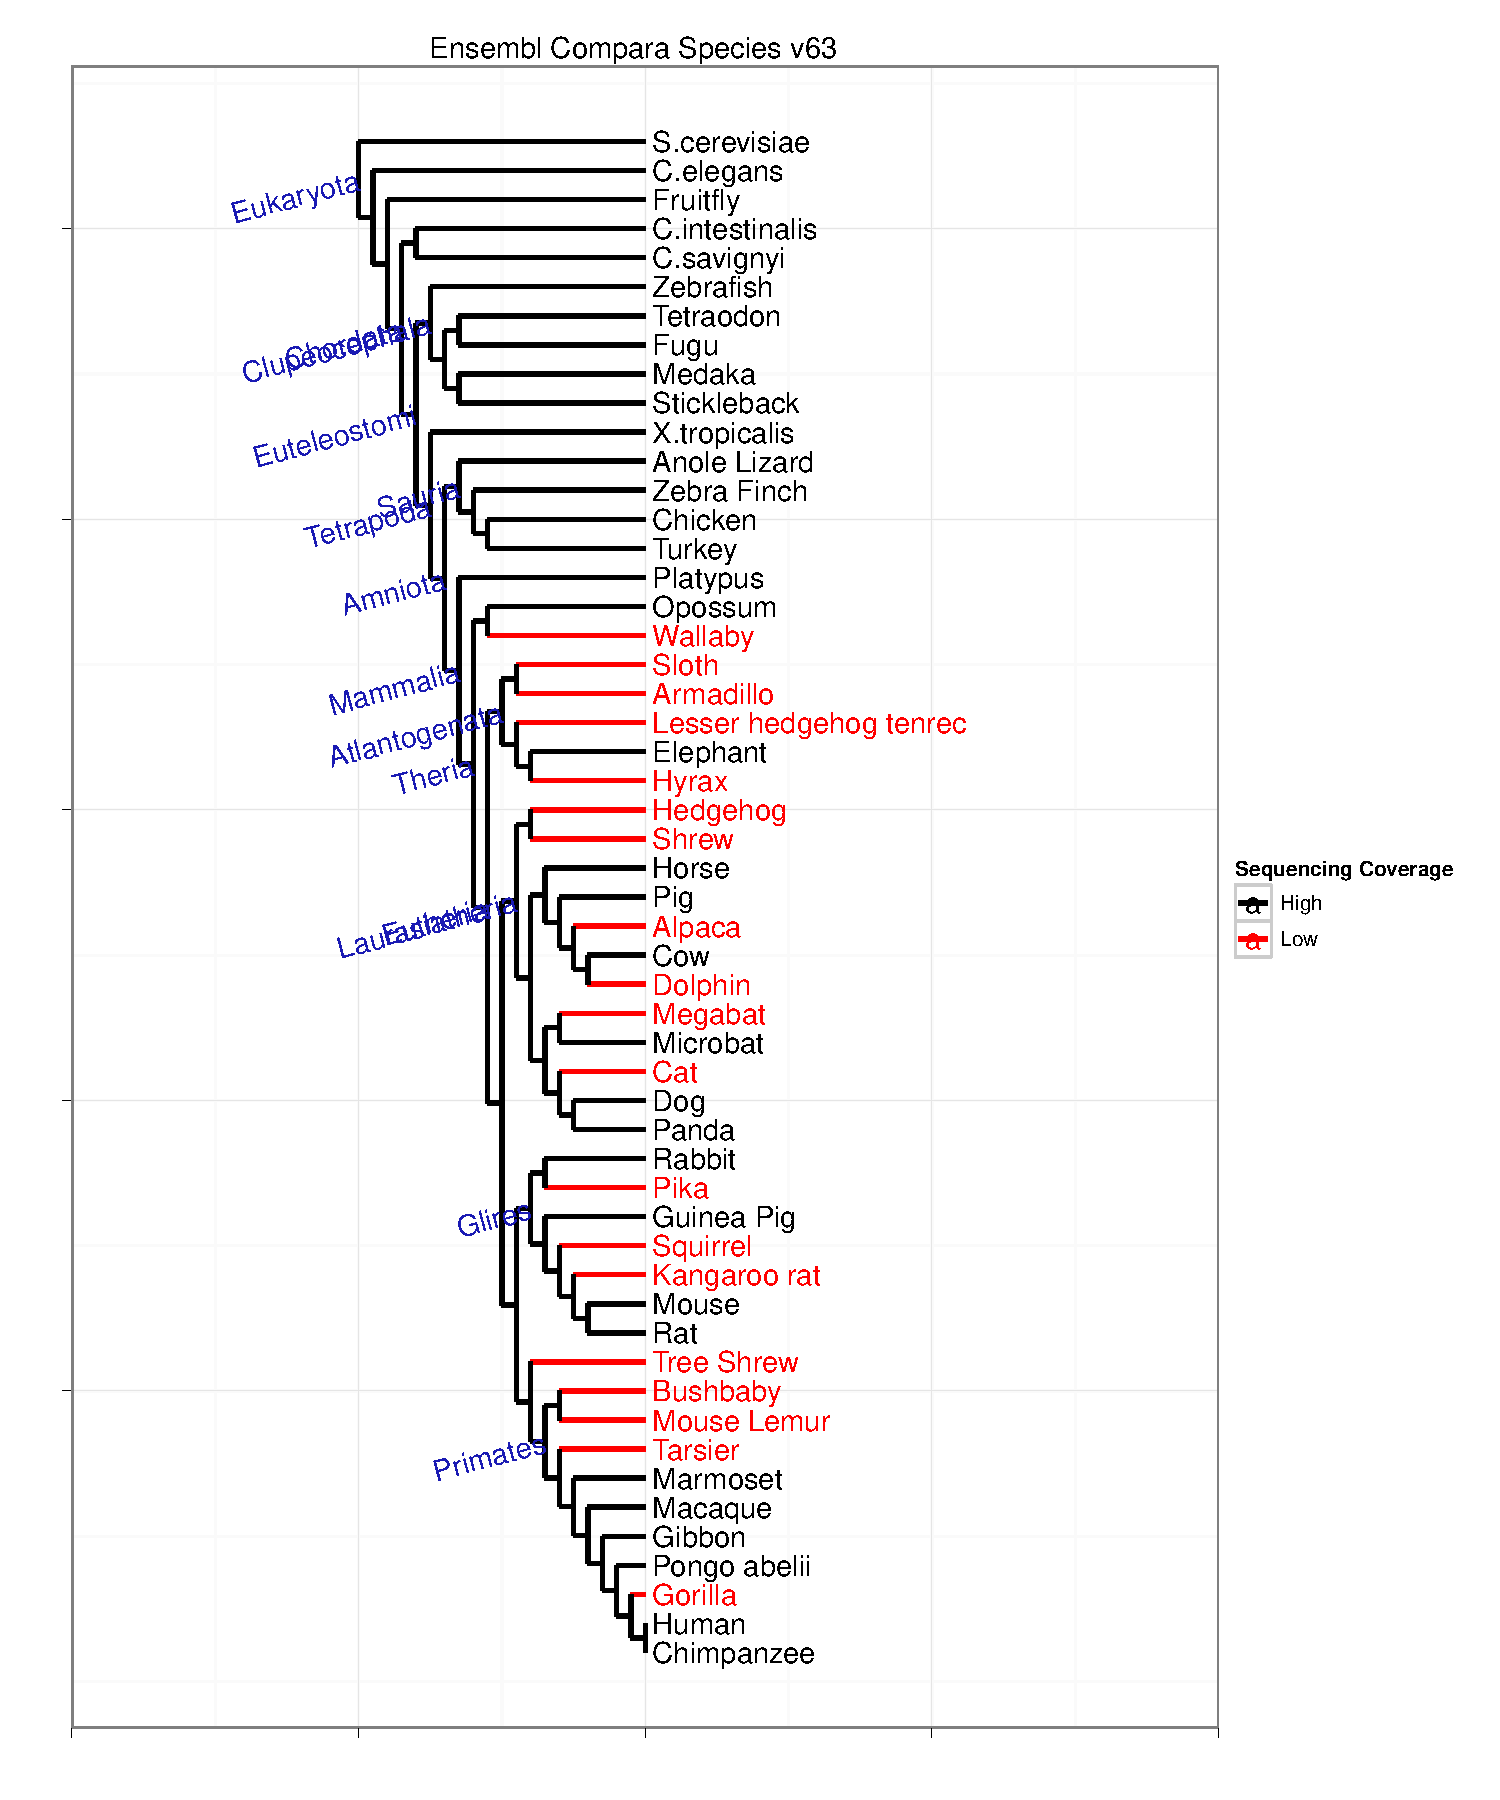
\includegraphics[scale=0.4]{Figs/compara_63_tree.pdf}
\caption{The NCBI taxonomy of species within the Ensembl Compara
  database. Note that branch lengths are not drawn to
  scale. Low-coverage genomes are labeled in red, high-coverage
  genomes are in black. Selected internal nodes, used are labeled in
  blue.}
\label{ncbi_tree}
\end{figure}


\begin{table}[ht] \footnotesize
\centering
\begin{tabular}{@{}lll@{}} \toprule
\multicolumn{2}{c}{Method} \\ \cmidrule(r){1-2}
   Category & Name & Constraints \\ \midrule
Ingroup & Primates & $TC(Primates) > 0.6$ \\
 &   Glires &  $TC(Glires) > 0.6$ \\
 &   Laurasiatheria & $TC(Laurasiatheria) > 0.6$ \\
 &   Sauria & $TC(Sauria) > 0.6$ \\
 &   Fish & $TC(Clupeocephala) > 0.6$ \\
Outgroup &  Eutheria & $TC(Eutheria) > 0.6$ \\
 &   Amniotes & $TC(Amniota) > 0.6$\\
 &   Vertebrates & $TC(Vertebrata) > 0.6$\\
 &   Fungi/Metazoa & $TC(Fungi/Metazoa) > 0.6$\\
Subgroups &  MammalSubgroups & $TC_{all}(Laur., Glires, Primates) > 0.1$\\
 &   MammalSubgroupsPlusOutgroup & $TC_{all}(Laur., Glires, Primates) > 0.1$ AND \\
 &    & $TC_{any}(Sauria, Clupeo., Ciona, Marsup.) > 0)$ \\
Orthologs & Human Orthologs & \\
 &   Mouse Orthologs &  \\
 &   Zebrafish Orthologs &  \\
 &   Drosophila Orthologs &  \\
Root Nodes & Ensembl Roots &  \\
\bottomrule
\end{tabular}
\caption{Subtree constraints used for identifying Eutherian
  orthologous subtrees. Ensembl gene trees were split into subtrees
  based on taxonomic coverage (TC) requirements at internal
  nodes. Laur. - Laurasiatheria; Clupeo. - Clupeocephala; Marsup. -
  Marsupiala}
\label{subtree_constraints}
\end{table}

\section{Analysis of genome-wide sets of orthologous mammalian trees}

The \subtr splitting schemes described in the previous subsection were
each applied to the 18,607 root gene trees from the Ensembl
database. In this and the next section I will describe the resulting
sets of trees and \subtr{}s, discuss what they reveal about the
evolutionary history of vertebrates and the feasibility of using
taxonomic coverage to isolate orthologous trees for sitewise analysis,
and finally, explain my reasoning for deciding to use the subtrees
based on the Eutherian taxonomic coverage for the subsequent sitewise
analysis.

\subsection{The set of root Compara gene trees}

Table \ref{ensembl_root_table} presents a summary of the set of root
Compara gene trees and the subsets of trees with more or fewer than 15
sequences.

\begin{table}[hb] \footnotesize
\centering
\begin{tabular}{lrb{2cm}rrrrrrr}
\toprule
Tree & &  Med. Size &  & \multicolumn{3}{c}{Human Content} & Human & Med. & Med. \\ \cmidrule(r){5-7}
Set & Count  & (Min / Max) & N50 & 0 & 1 & 2+ & Total & MPL & Species \\ 
  \midrule
\input{Tables/ortholog_roots_summary.txt}
   \bottomrule
\end{tabular}
\caption{Summary of the set of Ensembl Compara root trees. The 'Human
  Content' columns represent the fraction of trees which contain the
  indicated number of human genes, and 'Human Total' is the total
  number of human genes contained within the tree set. 'Med. Species'
  is the median species count across all trees. Med. - median, MPL -
  mean path length }
\label{ensembl_root_table}
\end{table}

It is somewhat surprising that nearly half of all Compara gene trees
contain few sequences: 9,378 out of 18,607 root trees constitute fewer
than 15 sequences. Given the protein-based clustering performed by the
Compara pipeline, one might expect many of these small trees to
represent portions of larger fast-evolving gene trees whose high
sequence divergences made the BLAST search step inaccurate or caused
clustering via the \hclust algorithm to be ineffective. Alternatively,
these small clusters might have resulted from exceptional
lineage-specific gene duplications or pseudogenes mis-annotated as
genes, creating tight clusters of very closely-related transcripts
that were identified by \hclust as independent gene trees. Some
evidence for the latter scenario comes from the median species counts
and mean path lengths of the smaller versus larger trees. The subset
of small root trees has a median species count of 2 compared to 47 for
the large subset, indicating that the smaller trees encompass
sequences from a very small taxonomic range. Furthermore, the median
MPL for small trees is 0.04 compared to 1.04 for the large subset,
revealing a much smaller level of sequence divergence within each
tree. Together, these summary statistics indicate that the smallest
trees in the Compara database consist of highly species-specific,
closely-related proteins that are likely artifactual gene
annotations.

Despite the existence of many small trees in the Compara database,
they comprise only a small fraction of all protein-coding
sequences. Only 4\% of the human gene set---which we expect to be
well-annotated and to contain few false positive genes due to the high
level of manual curation and the large amount of continued
scrutiny---is contained within the subset of small trees. This
indicates that whatever process is causing the Compara pipeline to
yield such a high number of small gene trees has not had too much of
an impact on the placement of the most confident set of protein-coding
genes within the database of root gene trees.

\begin{figure}[ht]
\centering
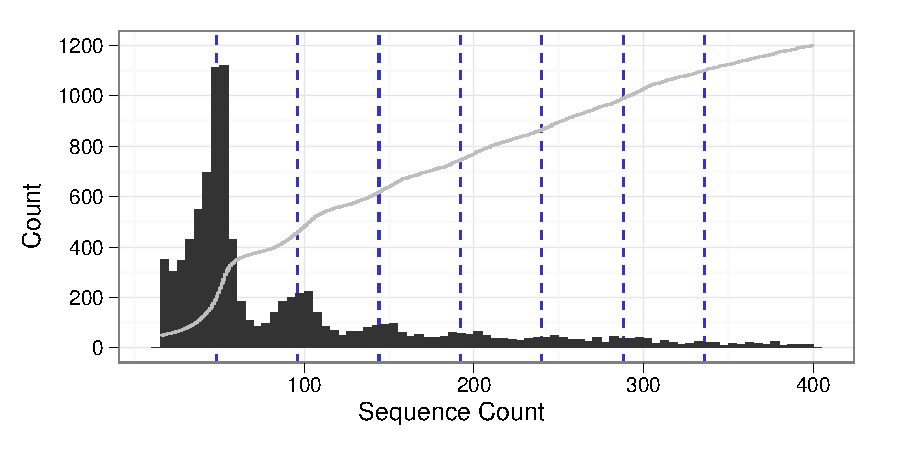
\includegraphics[scale=0.9]{Figs/ensembl_roots_hist.pdf}
\caption{Sequence counts for the set of root Compara trees. Black bars
  show a histogram of sequence counts in bins of width 5, and the gray
  line shows the cumulative fraction of sequences contained within
  trees of that size or smaller. For clarity, 9,378 trees with 15 or
  fewer sequences are not shown. Dashed green lines are drawn at
  integral multiples of 48, the number of vertebrate species within
  Ensembl.}
\label{ensembl_roots_hist}
\end{figure}

A closer examination of the distribution of tree sizes in the set of
root Compara trees presents a clear view of the over-clustering of
mammalian orthologous trees. The black bars in Figure
\ref{ensembl_roots_hist} show the distribution of sequence counts for
all trees with more than 15 sequences, with vertical dashed lines
overlaid at multiples of 48 (the number of vertebrate species in
Ensembl release 63). The highest peak
of the histogram is at or slightly above 48 sequences, with the tree
counts quickly diminishing at larger sizes. Weaker, but still
discernable, peaks appear at larger tree sizes, with the location of
these echo-like peaks corresponding closely to the second, third and
fourth multiples of 48. The pattern of recurring peaks becomes
indistinguishable at sizes above 200, but there is still a long tail
of large trees extending out to a maximum size of 400
sequences. Overall, the distribution of tree sizes provides good
support for the situation described above, with the Compara pipeline
often clustering together two or more largely-orthologous gene trees
sharing ancient homology.

It is also interesting to characterize the set of Ensembl trees by the
proportion of all sequences which are covered by trees of a given size
or smaller. This value is plotted in Figure \ref{ensembl_roots_hist}
as a gray line. First, one can see that trees with fewer than 15
sequences (which were excluded from the plot but inlcuded in the
calculation of the cumulative fraction of sequences) represent a
trifling fraction of the sequences within Compara; this is similar,
but not identical, to the above-mentioned calculation that 4\% of
human genes are contained within these smaller trees. Second, the
steady slope of the cumulative curve contrasts with the declining
height of the histogram. This results from the increasing number of
sequences encompassed by each of the larger trees: although there are
relatively few trees with more than 300 sequences, together they
contain around 10\% of all protein-coding genes in Ensembl. Two points
along this cumulative plot are of particular interest. First, one can
identify the fraction of vertebrate proteins which exist as
identifiable paralogs. Looking at the value along the x-axis where the
largest bump in the histogram ends, at around 75 sequences, one can
see that in total around 30\% of proteins are covered by trees of 75
sequences or fewer. Since the pattern of bumps in the histogram
correlate well with the number of Ensembl vertebrate species, it would
be reasonable to state that 70\% of vertebrate proteins are contained
within large gene trees containing sequence-based evidence of ancient
paralogy. Second, a look-up in the reverse direction can identify the
tree size at which 50\% of sequences are clustered. This value
represents the size of tree that an ``average'' protein might be
clustered in, and in some ways is a more accurate characterization of
the set of gene trees than the median tree size. A similar calculation
is often performed to characterize the size distribution of contigs
(contiguous sequence blocks) within a genome assembly. This statistic,
referred to as the N50 length, is the contig length for which 50\% of
bases are contained in contigs of that size or larger
\citep{TODO}. For the Ensembl root trees, the N50 tree size is 139,
slightly less than three times the number of vertebrate species. The
N50 tree size is shown for the root trees in Table
\ref{ensembl_roots_hist} and in the table for taxonomically-defined
tree sets below.

Another way to characterize the distribution of gene trees is across
the taxonomic space. A question of particular interest to the
identification and analysis of mammalian orthologs is whether levels
of gene presence and absence are consistent across different species
and different levels of assembly quality. To investigate this question
in the context of the root Ensembl trees, data were collected by
counting the number of sequences from each species contained within
each gene tree. Results were tabulated for each species and are
presented in Figure \ref{ortholog_root_dups}, showing the number of
trees containing 0, 1, 2, or more than 3 genes from each of the 53
species in Ensembl. Comparing the range of values in the panels for
each copy count (labeled 0, 1, 2 and 3+), one finds that most trees
(8,000-11,000 within vertebrates) contain zero copies from a given
species, fewer trees contain one copy (4,000-6,000) and several
thousand contain two, three or more copies (ca. 1,000-1,500 for 2
copies and 1,500-2,000 for 3+). The plethora of trees with zero copies
from a given species is again a result of the existance of many small,
species-specific trees within the root Ensembl set. Similarly, the
high number of trees with many copies from each species reflects the
clustering of multiple orthologous sub-trees together.

A comparison of values across the range of species in Figure
\ref{ortholog_root_dups} reveals that the zero-copy count tends to
increase along with evolutionary distance from human, while the 1, 2
and 3+ copy counts tend to decrease as the distance from human
increases. Both trends are most striking at the distant end of the
tree where the five non-vertebrate species begin. For the increase in
zero-copy trees and the decrease in single-copy trees, the strength of
the trend at the highest level of divergence can be partly explained
by the very long branch lengths connecting those species to each other
and to the more well-represented vertebrate clade: the distance-based
clustering algorithm might reasonably be expected to produce more
false negatives in longer branches for a number of reasons including
the behavior of the \hclust algorithm, inaccurate BLAST E-values at
larger distances, and heterogeneity in evolutionary rates across
lineages \citep{TODO}. However, the dearth of 2 and 3+ copy counts in
non-vertebrates is most likely a signal resulting from the 2R event at
the basal vertebrate lineage, with the non-vertebrate species strongly
depleted of multi-copy duplicates compared to their vertebrate
relatives.

It is slightly concerning that human and its close primate relatives
contain fewer zero-copy genes and more one-copy and two-copy genes
than any other group of vertebrates in the set of Ensembl trees. There
is no \emph{ab initio} biological reason to expect this to be the
case, and I suspect that the existence of such a pattern, which is
fairly small in effect, is due to the widespread reliance on human
annotation and protein experimental data in the annotation of
non-human genomes. There is one region where this trend does not
appear to be the case: in the 3+ copy count for the fish species,
which is instead a result of gene duplicates retained after the third
round of genome duplication which occurred in the teleost ancestor
\citep{TODO}. The signal resulting from the teleost genome duplication
event is clearer in the sets of taxonomically-defined \subtr{}s, so I
will defer its discussion to the next subsection where those sets of trees are described.

Finally, the differences in copy counts between species with low- and
high-coverage genome sequences show the tendency of low-coverage
genome sequences to yield false negatives in the gene annotation, as
low-coverage species contain more zero-copy, roughly the same number
of one-copy, and noticeably fewer multi-copy genes than high-coverage
species. These clear effects of low sequencing coverage show that gene
absence in low-coverage genomes should not be taken as evidence for
actual gene loss and that gene duplications are systematically
underrepresented in low-coverage genomes. The former point was
emphasized in a recent critical analysis of the effect of low-coverage
genomes on gene duplication inference \citep{TODO, Milinkovitch et
  al. 2010}, but the latter point was largely ignored. Again, this
signal is also stronger in the more stringent set of \mmln orthologous
\subtr{}s and will be revisited in the next subsection.

The preceding analysis of the set of root Ensembl trees, in which I
characterised the distribution of trees with respect to size
(i.e. sequence count) and across the taxonomic space, showed that
despite the over-representation of small, species-specific trees, most
sequences are contained in trees with biologically plausible sizes
given the history of vertebrate genome duplications. The tree-based
equivalent of the N50 statistic was developed for summarizing the
distribution of differently-sized trees, and two main views of this
distribution were introduced (in Figures \ref{ortholog_root_dups} and
\ref{ensembl_roots_hist}), providing evidence for the clustering of
paralogous mammalian sub-trees and for species-based and genome
coverage-based trends in the breakdown of gene copy counts within
these trees.

\begin{landscape}
\begin{figure}[ht]
\centering
\includegraphics[scale=0.9]{Figs/ortholog_root_dups.pdf}
\caption{Taxonomic distribution of gene copy counts for the root
  Ensembl trees. The number of trees containing 0, 1, 2 or more than 3
  sequences from each species is shown. Bars are colored blue and gray
  for species with high- and low-coverage genomes, respectively. Note
  that the y-axis scale is not the same for each panel.}
\label{ortholog_root_dups}
\end{figure}
\end{landscape}

\subsection{Sets of \subtr{}s defined by taxonomic coverage and orthology annotation}

The sets of trees resulting from applying the various \subtr
extraction methods to the root Ensembl gene trees are summarised in
Table \ref{ensembl_subtree_table}, with the original Ensembl trees
included at the bottom for comparison.

The Ensembl Roots and Drosophila Orthologs sets are two clear
outliers, with much higher N50 values than any other set (139 and 125
vs. the next highest value of 56) and more trees with multiple human
copies (0.20 and 0.43 vs. the next highest value of 0.14). In fact,
the major differences between these sets are all attributable to the
excess of small species-limited trees in the Ensembl Roots group: the
Drosophila Orthologs set contains fewer trees than the Ensembl Roots
(9,210 vs. 18,607) and a larger average tree size (60 vs. 15), closely
resembling the set of Ensembl Roots with small trees removed as
summarised in the third row of Table \ref{ensembl_root_table}.

Within the Ingroup category of methods, the methods based on
mammalian TC values (Primates, Glires and Laurasiatheria) produced
largely similar sets of trees, with the Primate set containing around
2,000 more trees and covering around 1,000 more human genes than the
other two sets. A reason for the higher number and human coverage of
Primate trees is not immediately apparent, although it may
speculatively be due to an excess of primate-specific gene trees that
are not captured by non-primate TC-based criteria. Further
investigation of the trees unique to this set might reveal the root
cause of this slight discrepancy.

The Sauria and Fish tree sets stood in strong contrast to the
mammal-based methods from the Ingroup category. The Sauria clade is
represented by only four Ensembl species and diverged from the
mammalian ancestor at an early point in the evolution of amniotes. The
moderately lower number of trees (13,046 vs. 15,764 for
Laurasiatheria) and the increased proportion of trees containing
multiple human genes (0.14 vs. 0.09 for Laurasiatheria) are presumably
consequences of the lower clade size, which could affect the TC
calculation, and the long branch separating Sauria from the other
vertebrate clades. The fish-based subtree constraint produced a
strikingly different set of trees resulting from the impact of the
teleost-specific whole genome duplication on the structure of fish
gene trees. Although the Fish tree set contains a N50 value of 49
which is no different from the N50 of the other Ingroup sets, Table
\ref{ensembl_subtree_table} highlights three major differences in the
Fish set: it contains many more trees, a higher proportion of trees
with zero human copies, and a lower total human gene count than the
other Ingroup sets.

The reason for the drastically different Fish tree set is that the
tree splitting procedure identifies largest non-overlapping \subtr{}s
that satisfy the given TC criteria. Genes that were duplicated in the
teleost lineage and retained in duplicate form (as opposed to one or
both copies being lost in either of the descendant duplicate
chromosomes) would result in a gene tree with two teleost-specific
\subtr{}s, each containing a high TC value for the Clupeocephala
clade. In this case, the splitting procedure would result in two small
Fish subtrees, ``missing'' the single subtree of mammalain orthologs
because two non-overlapping trees already exceeded the TC threshold of
0.6. If, however, one of the duplicate gene copies were lost, then the
tree would resemble a typical singly-orthologous vertebrate gene tree,
and the splitting procedure would select a \subtr encompassing the
entire vertebrate clade. It follows that the presence of small,
teleost-specific gene trees in the Fish set is a signal of retained
duplicate copies, and the size distribution of trees from the Fish
set, shown in Figure \ref{ensembl_fish_hist}, shows that several
thousand trees fit the expected model. If we assume that all trees
from the Fish subset which contain zero human copies, span 5 or fewer
species, and contain 40 or fewer sequences are likely retained
duplicate genes, a total of 6,980 retained duplicates are identified,
yielding a retention rate of 17.5\%, which is very much in line with a
previously published estimate of 15\% based on a comparison of
tetraodon, fugu and zebrafish genes \citep{TODO, Brunet et al. MBE
  2006}.

\begin{figure}[ht]
\centering
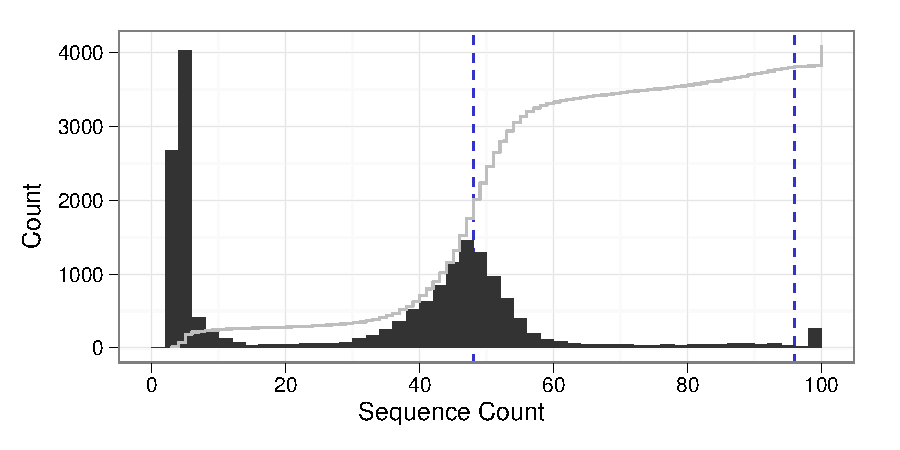
\includegraphics[scale=0.9]{Figs/ensembl_fish_hist.pdf}
\caption{Sequence counts for the set of \subtr{}s identified using the
  Fish clade taxonomic coverage constraint. Black bars show a
  histogram of sequence counts in bins of width 2, a gray line shows
  the cumulative fraction of sequences contained within trees of that
  size or smaller, and dashed blue lines are drawn at integral
  multiples of 48, the number of vertebrate species within
  Ensembl. The 255 trees with more than 100 sequences are not shown.}
\label{ensembl_roots_hist}
\end{figure}


The sets of \subtr{}s resulting from the Outgroup methods were of
special interest, as the clades used to define these TC constraints
contained all or nearly all of the mammalian species whose orthologous
genes I wished to study. The resulting sets of \subtr{}s show little
variation, owing perhaps to the large sizes of the clades and their
similar composition. Each set contained between 15 to 17 thousand
trees, N50 values of around 49, and greater than 90\% of trees
containing exactly one human sequence. These measures provided good
evidence that the tree-splitting method was effectively isolating
singly orthologous mammalian trees.  Some slight trends were apparent,
however, with the tree count decreasing, the proportion of trees with
human duplications increasing, and the overall human gene coverage
decreasing as the clade size used for the TC calculation
increased. These trends could understandably be the result of the
minimum required tree size increasing along with the clade size,
ranging from 21 for Eutheria to 32 for Fungi/Metazoa.

The Subgroups methods did not appear to produce \subtr{}s of any
higher quality or more biological interest than the Outgroup
methods. The MammalsSubgroups set was more numerous than the Outgoups
sets, but the N50 was slightly lower (46 vs. 49) and the proportion of
zero-humany trees was higher (0.18 vs. 0.01), suggesting that the
additional trees were spurious results containing fragmented species
coverage. The addition of an outgroup requirement to the
MammalSubgroupsPlusOutgroup method produced a tree set more closely
resembling the Outgroup methods, but the human gene coverage was
lower than that for any Outgroup method despite the overall higher
tree count.

Finally, the ortholog annotation-derived \subtr{}s provided for an
interesting comparison between three different ortholog sources and
between the overlapping and non-overlapping sets of \subtr{}s. As I
mentioned at the beginning of this section, the \species{Drosophila}
ortholog set was highly contrasted with the vertebrate sets due to the
two rounds of whole genome duplication. There was minimal variation
among the other ortholog sets, although it is interesting to note that
Ensembl contained 21,873 mouse protein-coding genes while human
contained only 19,991. Zebrafish, on the other hand, contained 24,540
genes, in line with the 17.5\% rate of duplicate gene retension I
estimated earlier. Overall, 76\% and 81\% of mouse and zebrafish genes
have an apparent one-to-one ortholog in human, which is slightly lower
than the 92\% of Eutheria \subtr{}s containing one human sequence.

\begin{landscape}
% latex table generated in R 2.13.0 by xtable 1.5-6 package
% Thu Sep 15 11:19:59 2011
\begin{table}[ht]
\centering
\begin{tabular}{llrb{2.5cm}rrrrrrr}
\toprule
\multicolumn{2}{c}{Method} & &  Med. Size &  & \multicolumn{3}{c}{\% w/ Human Count} & Human & Med. & Med. \\ \cmidrule(r){6-8} \cmidrule(r){1-2}
Category & Name & Count  & (Min / Max) & N50 & 0 & 1 & 2+ & Total & MPL & Species \\ 
  \midrule
\input{Tables/ortholog_summary.txt}
\bottomrule
\end{tabular}
\caption{Summary of Ensembl \subtr{}s identified using taxonomic
  criteria or Ensembl ortholog annotations. The set of Ensembl root
  trees (``Ensembl Roots'') from Table \ref{ensembl_root_table} is
  included for comparison. Cells in numeric columns are shaded
  according to their value relative to other rows, with low values in
  white and high values in blue. The 'Human Content' columns represent
  the fraction of trees which contain the indicated number of human
  genes. 'Med. Species' is the median species count across all
  trees. Med. - median, MPL - mean path length}
\label{ensembl_subtree_table}
\end{table}
\end{landscape}

Figure \ref{ortholog_stacked_bar} shows the taxonomic distribution of
gene copy counts for the trees resulting from each of the \subtr
methods tested. By way of reference, the values shown in the separate
panels of Figure \ref{ortholog_root_dups} appear in Figure
\ref{ortholog_stacked_bar} as different-colored bars in the bottom
panel. Although the various characteristics of each of the \subtr
methods have already been discussed at length, the taxonomic view
reveals some salient features of the patterns of gene deletion and
duplication within the tree sets and shows the pervasive impact of
genome-wide duplications on the evolution of vertebrate genes. The
large fraction of species with multiple copies in Drosophila Orthologs
\subtr{}s is a result of the two rounds of vertebrate genome
evolution, while the elevated fraction of multi-copy fish trees in the
Outgroup \subtr{}s shows the impact of the teleost-specific
duplication event.

Furthermore, the relative prevalence of zero-copy and multi-copy trees
can provide some indication of whether gene deletion or gene
duplication is a more common process in vertebrate genomes. Focusing
on the four Outgroup \subtr methods, the observation of a greater
number of multi-copy trees than zero-copy genes, valid across all four
\subtr methods and throughout all mammalian species except platypus,
can be interpreted as tentative evidence for a greater number of gene
duplications than gene deletions in the evolution of mammalian
genomes. This pattern does not hold for vertebrates more distantly
related to human, however: vertebrates beyond opossum show a distinct
and consistent increase in zero-copy trees, and birds appear to
exhibit a slight clade-specific drop in the proportion of multi-copy
trees. Of course, both of these trends could be methodological
artifacts related to the \hclust algorithm or to the methods used to
assemble and annotate more distantly-related genomes.

The distributions in Figure \ref{ortholog_stacked_bar} also reveal the
pig to harbor a very high number of apparent gene deletions, unmatched
by other mammalian species and nearing the proportion of zero-copy
trees seen in platypus and more distant vertebrates. Given the
consistently low proportion of zero-copy trees for other
closely-related species, I would expect this number to change once a
finished-quality pig genome sequence is included in the Ensembl
pipeline \ref{TODO, Archivald et al. 2010}.

\begin{figure}[hb]
\centering
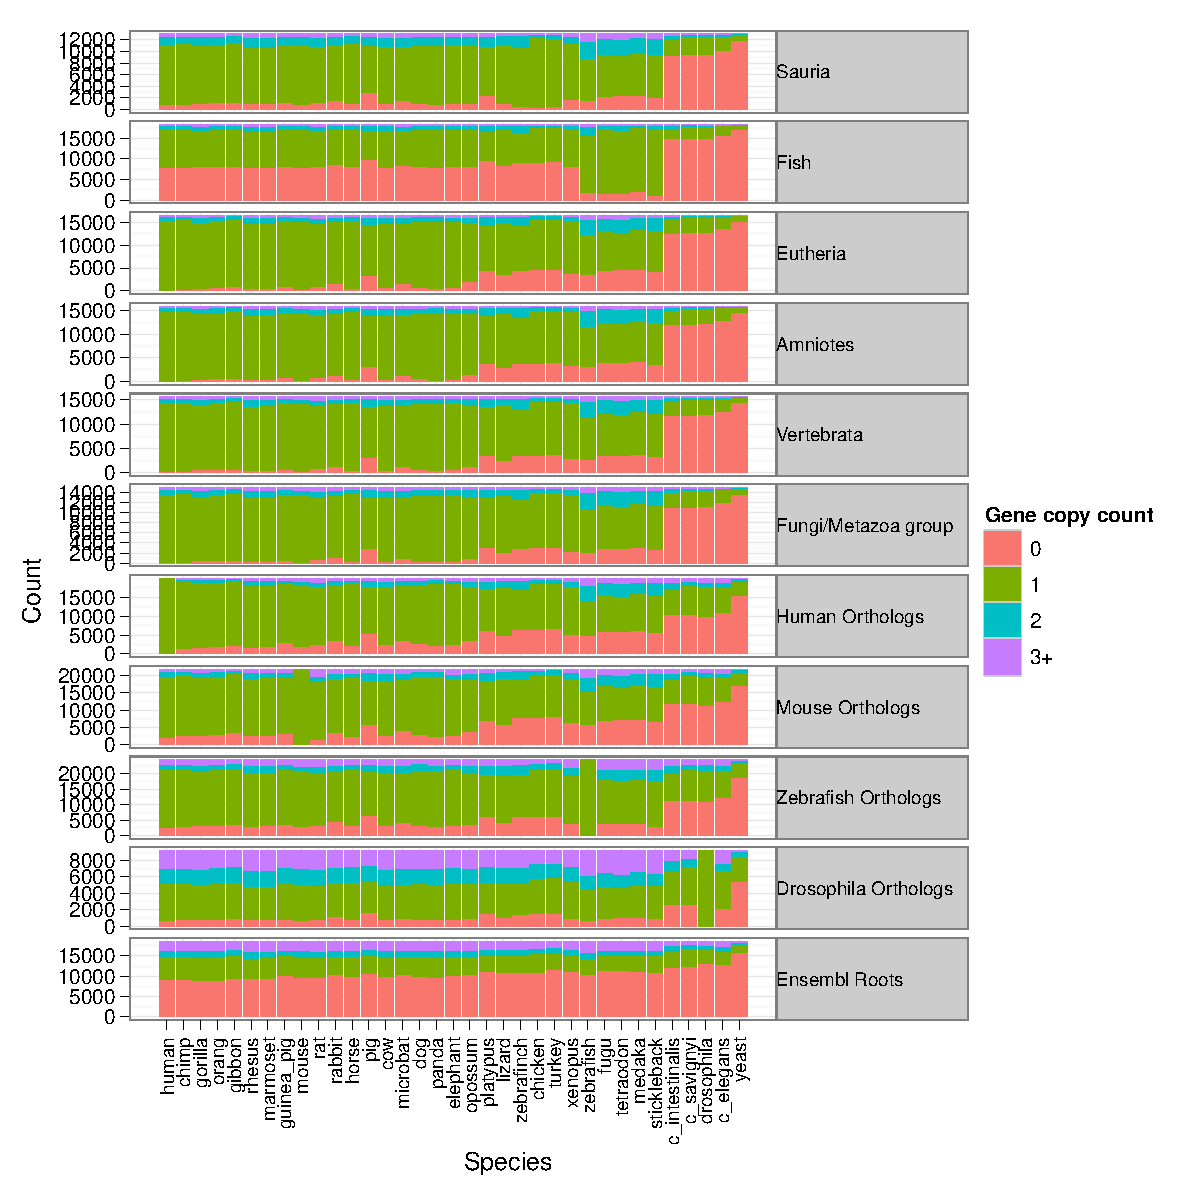
\includegraphics[scale=0.7]{Figs/ortholog_stacked_bar.pdf}
\caption{Taxonomic distribution of gene copy counts for different
  \subtr methods. The numbers of trees containing 0 (red), 1 (green),
  2 (blue) or more than 3 (purple) sequences from each species are
  shown as stacked colored bars. The Ingroup and Subgroups methods
  were omitted for clarity, as were species with low-coverage
  genomes. Note that the y-axis scale is not the same for each panel.}
\label{ortholog_stacked_bar}
\end{figure}

In the end, the set of Eutheria \subtr{}s was chosen as the final set
for use in the downstream evolutionary analysis, due to the slightly
larger number of trees and better coverage of human genes in the
Eutheria set compared to the other Outgroup methods. The distribution
of tree sizes for the Eutheria set of \subtr{}s is shown in Figure
\ref{ensembl_euth_hist} and the full taxonomic distribution of copy
counts is included in Figure \ref{ortholog_euth_dups}.

\begin{landscape}
\begin{figure}[ht]
\centering
\includegraphics[scale=0.9]{Figs/ortholog_euth_dups.pdf}
\caption{Taxonomic distribution of gene copy counts for the Eutheria
  \subtr{}s. The number of trees containing 0, 1, 2 or more than 3
  sequences from each species is shown. Bars are colored blue and gray
  for species with high- and low-coverage genomes, respectively. Note
  that the y-axis scale is not the same for each panel.}
\label{ortholog_euth_dups}
\end{figure}
\end{landscape}

\section{Preparing mammalian alignments for sitewise analysis}

As discussed in the introduction to this chapter, the effects of
sequencing, annotation and alignment error on the results of
comparative evolutionary analyses can be severe \citep{TODO}, with a
high potential for false positive results when using sensitive
evolutionary models \citep{TODO}. In order to minimize the potential
for false positive results in this study, sequences were prepared for
input to SLR with a series of filters and realignment steps designed
to (a) remove low-quality sequences prone to high error rates, (b)
realign sequences using an aligner with better performance for
detecting sitewise positive slection, and (c) mask out short alignment
regions with dubious elevated rates of nonsynonymous substitution. 

\subsection{Filtering out low-quality genome sequence}

Due to the presence of several low-coverage genome assemblies in the
set of available mammalian genomes and the elevated sequencing error
rates in such assemblies \citep{TODO, Ensembl 2x paper}, I applied a
conservative filter to the set of input sequences based on sequence
quality scores where available.

Most automated genome assembly pipelines, such as the Arachne tool
used to sequence many of the low-coverage mammalian genomes included
in Ensembl \citep{TODO, Arachne}, output a set of Phred quality scores
alongside the genome sequence, with one Phred score per base ranging
from 0 to 99. A Phred score represents the probability, calculated by
the sequencing and/or assembly program, that a given base call is
incorrect. This probability is usually concisely expressed as the
negative logarithm of the probability of an error multiplied by ten,
or $Q = -10log_{10}P$ where $Q$ is the Phred score and $P$ is the
probability of an incorrect base call \citep{TODO, Cock et al. 2010
  NAR}.

Unfortunately, Ensembl does not store quality scores from its source
genome assemblies, so Phred quality scores were downloaded for all
genomes with readily available Phred-like quality scores (\TODO{make a
  list of genome assemblies and quality score sources}). Most quality
scores were provided as a single file in FASTA format with one string
of numerical scores per assembled contig. Since the process of
filtering a mammalian coding alignment required collecting scores from
many different species at many disjoint genomic locations, an index
file was created for each quality score string based on the contig
name and sequence position to allow for quicker score lookup and
retrieval.

A suitable score threshold for filtering coding regions was chosen
based on the work of Hubisz et al. \citeyearpar{TODO}, who performed a
detailed analysis of Phred quality scores and observed error rates in
low-coverage mammalian genome assemblies by comparing the low-coverage
assemblies to matched regions of high-quality sequence from the ENCODE
comparative genomics dataset \citep{TODO}. The authors identified a
strong correlation between Phred scores and error rates for scores
below 25, indicating that the scores were accurate in this
range. Error rates did not decrease significantly at scores above 25,
however, suggesting that the value of using an extremely high Phred
score threshold would be minimal. Furthermore, Hubisz et al. noted
that 85\% of bases in the low-coverage mammalian genomes contain very
high Phred scores (>45) and only 4\% have low scores (<20).

Based on these considerations, a threshold Phred score of 25 was
chosen as a reasonable trade-off between the potential benefit of
avoiding miscalled bases and the potential cost of masking out
correctly sequenced bases. For each coding sequence (CDS) with quality
scores available, a ``minimum score'' approach was used to filter
codons: all codons containing one or more nucleotides with a score
below 25 were masked out with three ambiguous nucleotides,
'NNN'.

The expected proportion of filtered nucleotides can be calculated from
the fraction of bases below the Phred score threshold of 25. According
to the cumulative distribution of quality scores found in Hubisz et
al. \citeyearpar{TODO}, approximately 5\% of bases in low-coverage
mammalian genomes contain Phred scores below 25. The worst case
scenario, in terms of high-quality bases being masked as a result of
using the minimum score, would be if only one base per codon had a
score below the threshold. Were that the case, an expected 15\% of
nucleotides would be filtered, since 3 bases would be masked for every
low-quality base. However, the distribution of low-quality bases is
likely highly clustered, due to the uneven distribution of
repetitiveness and GC content as well as the tendency for uncertain
base calls to occur towards the end of sequence reads (all of which
are known to affect read coverage and assembly performance,
e.g. \cite{TODO, Teytelman et al. 2011}). A more clustered
distribution of low-quality bases would cause fewer high-quality bases
to become masked by the minimum score approach, reaching the limit of
5\% total filtered bases if they always occurred in codon
triplets. Thus, anywhere from 5\% to 15\% of low-coverage nucleotides
were expected to be filtered by this approach.

\TODO{Collect the filtering results and show a graph / some numbers on
  the amount of filtered material. How many genes had lots of filtered
  stuff? None at all? Which species were filtered the most?}

%\subsection{Realigning coding sequences}


%\subsection{Removing recent paralogs}


%\subsection{Filtering out clusters of \nsyn substitutions}



%\section{Results}


%\subsection{Analysis of the global distribution of mammalian selective pressures}



%\subsection{Analysis of sitewise estimates from three mammalian sub-clades}



%\subsection{Evaluation of the effect of GC content, recombination rate, and codon usage on sitewise dnds estimates and the detection of positive selection}


%\section{Conclusions}

